% \begin{figure*}[t]
% \centering
% 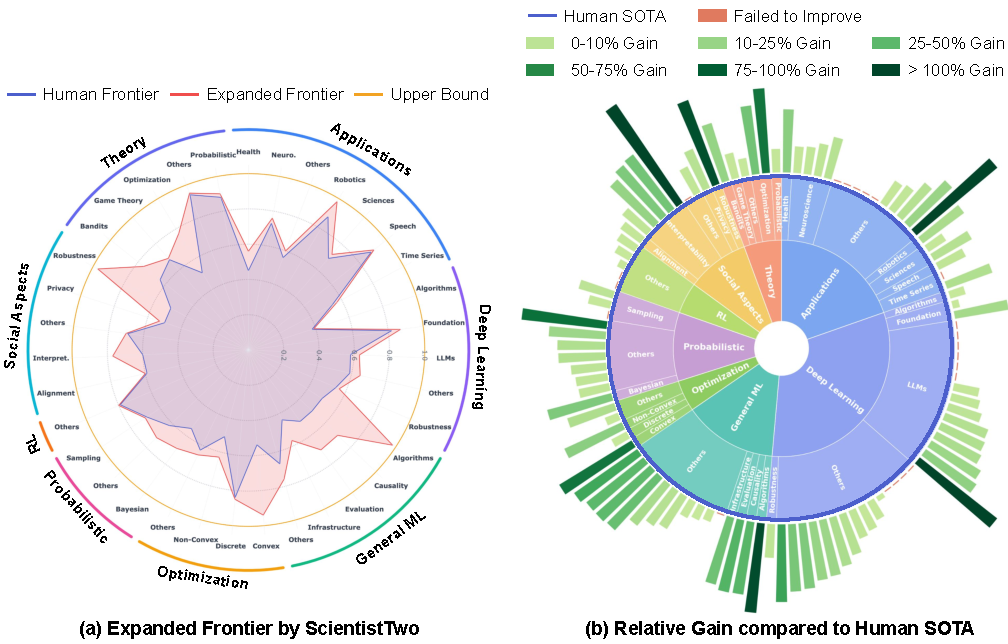
\includegraphics[width=\linewidth]{figures/sc2_new_fig2.pdf}
% \caption{\textbf{Problem setup.} \sname~automatically pushes the boundaries of human knowledge frontier by generating publication-quality papers and fully verified codebases, with resulting proposed novel methodologies consistently outperform human state-of-the-art baselines.}
% \label{fig:problem_setup}
% \end{figure*}
\begin{figure*}[t]
\centering
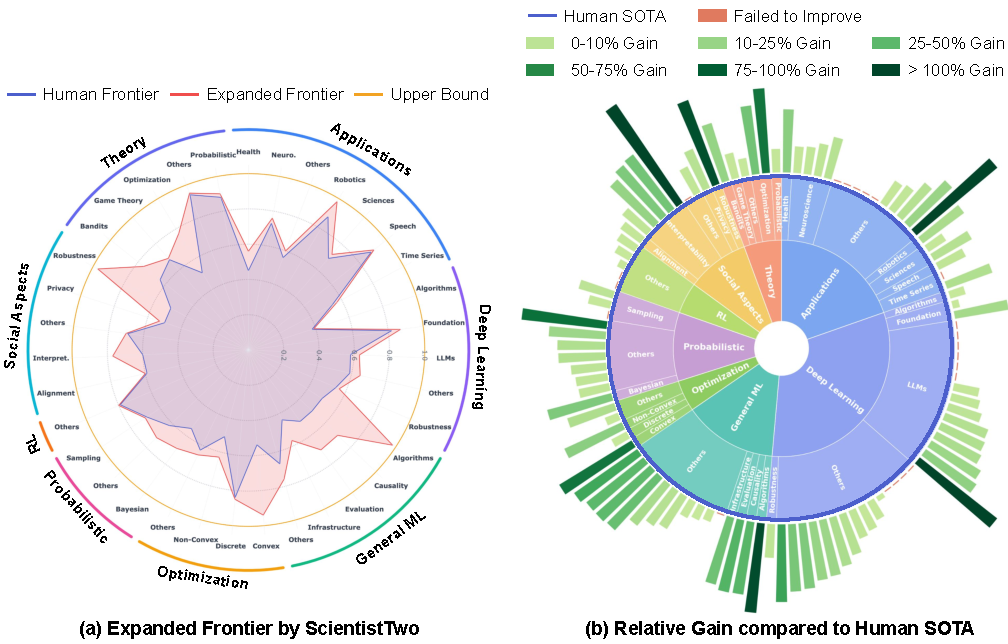
\includegraphics[width=\linewidth]{figures/sc2_new_fig2.pdf}
\caption{\textbf{Teaser.} \sname~pushes the frontier of human knowledge across diverse research domains (e.g., LLMs, robotics, neuroscience, speech, robustness, reinforcement learning, game theory, privacy, optimization, and time series) by generating publication-quality papers and fully verified codebases, with the resulting methodologies consistently outperforming human state-of-the-art baselines. Specifically, \sname~improves 86 out of 107 papers (an 80.4\% success rate) with an average relative improvement of 25.2\% over human state-of-the-art methods. Furthermore, papers generated by \sname~surpass the average scores of accepted papers at ICLR 2026 and NeurIPS 2025 under the Stanford Agentic Reviewer, demonstrating its capability to produce manuscripts that reach the empirical acceptance standards of top-tier AI venues.}
\label{fig:problem_setup}
\end{figure*}